\chapter{\label{detchar}Detector Characterisation with SOAP}
%%%%%%%%%%%%
%%%%%%%%%%%%
%%%%%%%%%%%%
%%%%%

When searching for \gls{GW} signals, it is important to understand the origins
of noise artefacts in the detector data which do not originate from an
astrophysical source.  A large fraction of \gls{GW} search algorithms,
including SOAP in Sec.~\ref{soap}, assume that the detectors noise follows a Gaussian
distribution~\chris{we don't totally assume that, e.g., the line aware stat you
have already discussed}.  However, the detectors contain artefacts which do not follow
this distribution.  These artefacts can negatively affect many searches for
\glspl{GW} as they can be easily mistaken for a real \gls{GW} signal.  Some of
the potential sources of these artefacts have been mentioned in
Sec.~\ref{intro:detector:noise}.  There are many different classes of artefact,
including: glitches, which are short duration broad band bursts in
power, and
instrumental lines, which are long duration narrow-band signals.  To conduct a
reliable search there are two main tasks which are necessary for detector
characterisation.  The first is identifying the artefact such that any search
knows which frequency bands and time segments are contaminated.  The search can
then address that section of data, this could mean removing that section of
data or using more sophisticated techniques to deal with the artefact
\citep{pankow2018MitigationInstrumental}.  The second task is to find the
instrumental or environmental source of the artefact.  If the source of the artefact is found, it can
potentially be removed or limited for future data runs.

The focus of this chapter is on how to search for and identify instrumental lines, and how this can improve the sensitivity of \gls{CW} searches.
Sec.~\ref{detchar:lines} will introduce different sub-classes of instrumental line and how each of them affects a \gls{CW} search.
Sec.~\ref{detchar:monitor} will outline how these artefacts are detected and monitored, and describe current tools used for this task.
Sec.~\ref{detchar:soap} will describe how the \gls{CW} search algorithm
introduced in Sec.~\ref{soap} can be used to search for instrumental lines.
Finally Sec.~\ref{detchar:summary} will describe the user interface for investigation SOAP's output.



%%%%%%%%%
%%%%%%%%%%
\section{\label{detchar:lines}Instrumental lines}
%%%%%%%%%
%%%%%%%%%

%
% Introduce instrumental lines

Instrumental lines can be generally described as persistent noise
artefacts.  There are many classes of
instrumental line spanning a range from narrow, fixed frequency spectral
artefacts to broader ($<0.1$ Hz) features which have a time varying frequency
known as wandering lines.  For many of these lines, it is difficult to
distinguish them from an astrophysical signal.  They affect search methods in
two main ways.  They can cause the search to produce outliers which are then
considered as \gls{GW} candidates.  Extra efforts then have to be made to
analyse these outliers further.  If the line is close to or overlapping with the \gls{GW}
frequency, then it can conceal the power of the \gls{GW}. 
Lines can also affect searches for \glspl{CW} by giving an incorrect estimate of the noise floor of the detector.
In searches for the \gls{SGWB}, channel data from multiple detectors is cross-correlated to identify a potential signal \citep{allen1999DetectingStochastic}.
If there is a noise source such as an instrumental line which is coherent between the detectors, this will show up as an excess in the cross-correlation statistic\citep{covas2018IdentificationMitigation}.
Any noise source which is local to both the detectors could then be visible in this cross-correlation.
It is therefore crucial to understand the structure and origin of these lines when performing a search for
\gls{GW}, specifically \gls{CW} and stochastic searches.

%
% What lines look like and how the appear in the GW channel

Some instrumental lines are clearly visible when looking at a \gls{ASD} or
\gls{PSD} of the \gls{LIGO} detectors. Figure \ref{detchar:line:psd} shows the
\gls{ASD} for \glspl{LIGO} Hanford and Livingston detectors during their first
observing run (O1) \citep{GWOpen}. This clearly shows peaks which are
associated with strong lines, where some of these have been labelled. There are however, many
more weaker lines which become visible when spectra are averaged over longer
times.
%
\begin{figure} \centering
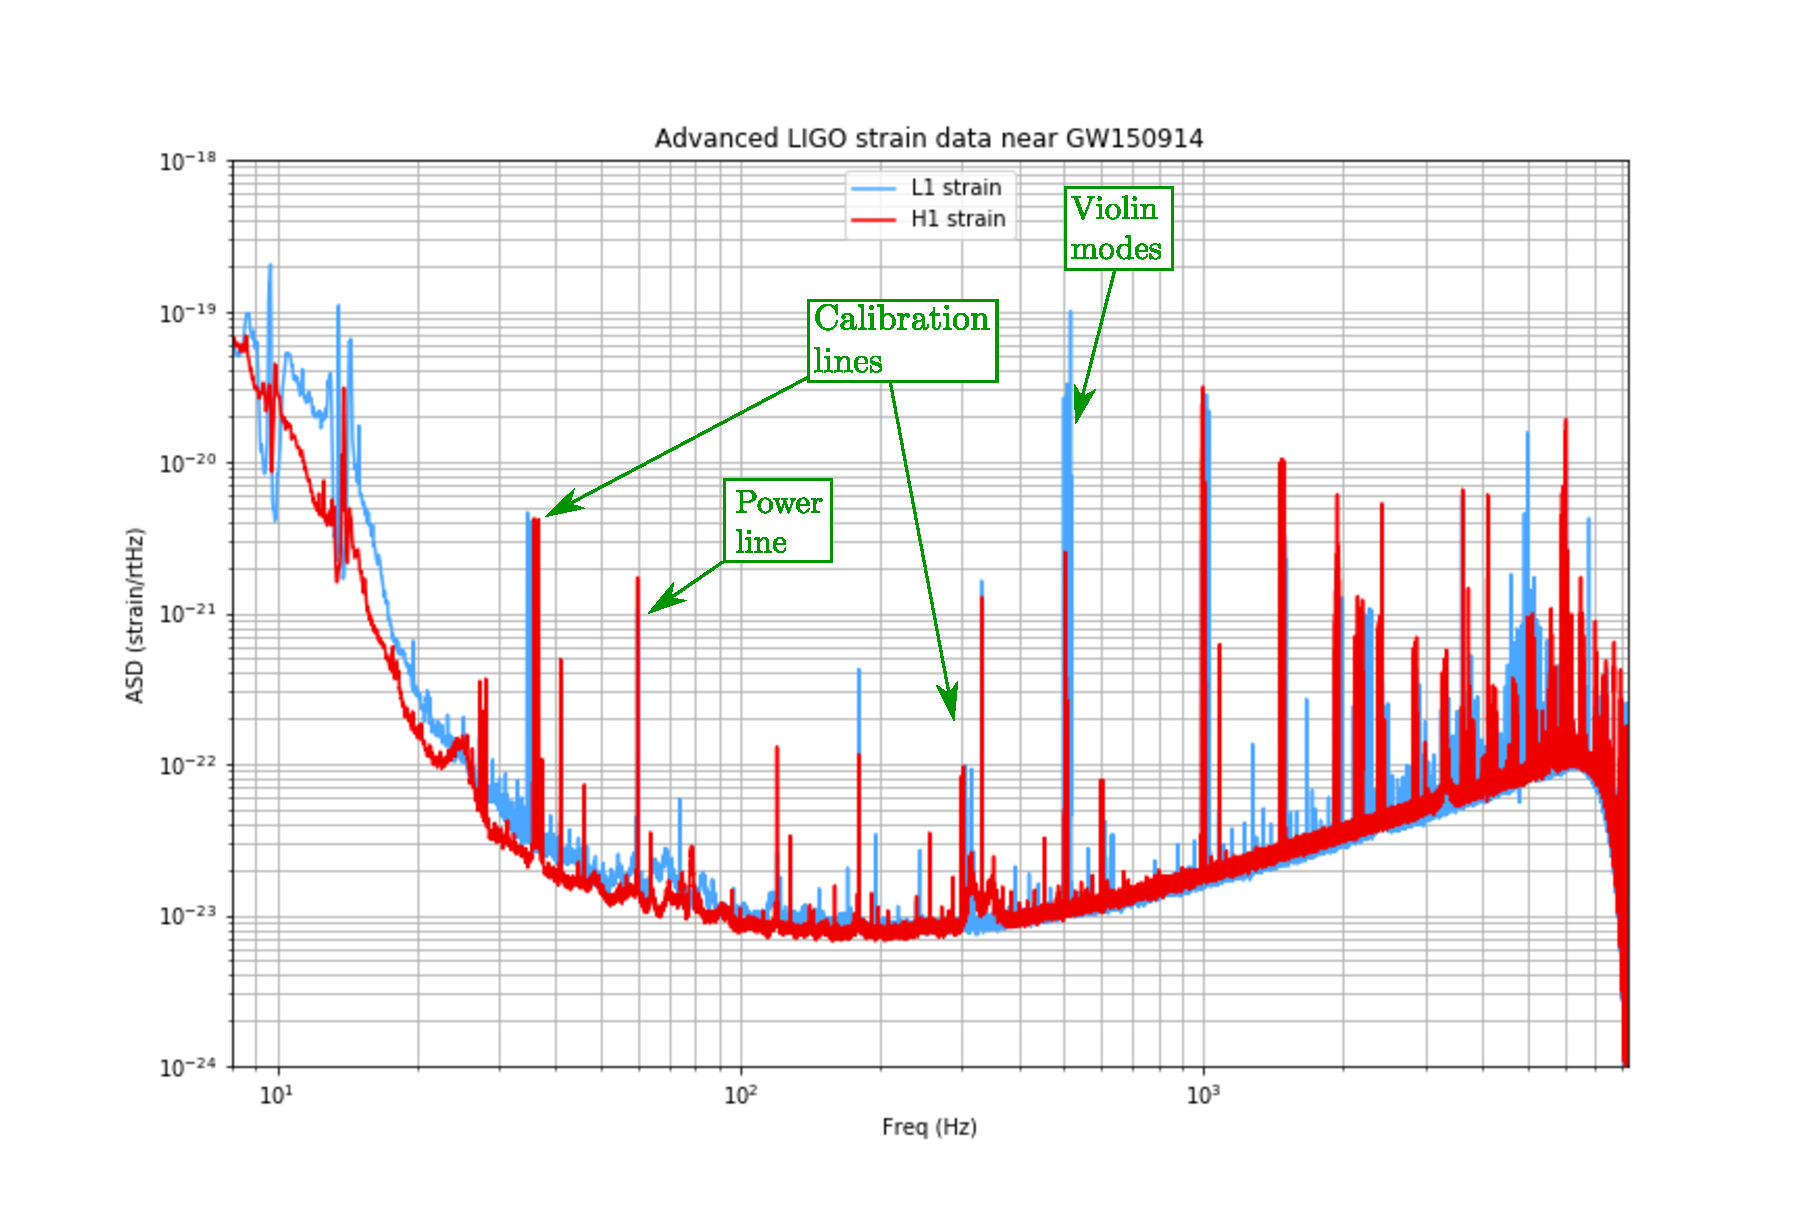
\includegraphics[width=\textwidth]{C6_detchar/ligo_o1_asd_annot.pdf}
\caption[Strain \gls{ASD} for the \gls{LIGO} detectors.]{
	The \gls{LIGO} detectors averaged \gls{ASD} is shown around the GW150914 event in O1 \citep{abbott2016ObservationGravitational}.
	This figure is from \citep{GWOpen} where the Power lines, Calibration lines and Violin modes are annotated. The
	power line from the mains in the USA is at 60 Hz. Some of the calibration lines
	are around 30 Hz, 331 Hz and 1083 Hz. The various violin modes of the suspensions are at 300, 500, 600 and 900 Hz where I have only marked the 500 Hz mirror suspension modes \citep{GWOpen}.} 
	\label{detchar:line:psd} 
\end{figure}
%
The \gls{ASD} in Fig.~\ref{detchar:line:psd} shows the time averaged spectra
of the \gls{GW} channel of the \gls{LIGO} detectors. The lines seen in the spectrum are not from any \gls{GW}
and are usually from terrestrial sources.  To see the lines in the \gls{GW}
channel, they must be transferred via some mechanism to this channel, known as coupling in.  There are a number of
ways in which this happens which are outlined in
\citep{covas2018IdentificationMitigation}.  This includes coupling via shared
power sources and shared grounds or earth's in the electrical circuits.  When different components share the same power supplies, if
a component draws power with a given period, then the voltage will decrease
repeatedly at this frequency.  Another component which shares this same power
supply can then also see this drop in voltage and this can potentially become
visible in a recorded output.  Another mechanism is coupling through magnetic
fields, this is common when cables are close to each other, the magnetic field
in one can affect the other, therefore, coupling noise between different
systems.  Coupling can also occur though a physical connection, known as
mechanical coupling, for example the resonances of the suspension fibers which
couple directly into the mirrors and therefore the output error signal.

%
% Origins of some lines and how they can be mitigated

Many of the spectral lines seen in the frequency spectrum in
Fig.~\ref{detchar:line:psd} are fundamental to the design of the detector.
These are difficult to eliminate at their source, therefore need to be understood such that their
effect on searches is minimised.  Some of the strongest of these lines are
listed below:

\begin{description}
	\item[Power line] The power line harmonics are fundamental to the
	detector and originate from the mains power supply in the
	\gls{USA}. These lines exist at 60 Hz which is the frequency of the
	mains alternating current \citep{aasi2015CharacterizationLIGO}. The European
	detectors Virgo and GEO have a power line at 50 Hz instead of 60 Hz.
	
    \item[Violin modes] The violin modes are associated with the
	suspensions fibers of the mirrors and the beam splitter in the detector. These are
	designed to have a narrow frequency spectrum such that they contaminate as
	small a part of the spectrum as possible. These are the lines around 500 Hz for
	the mirrors and 300, 600 and 900 Hz for the beam-splitter \citep{GWOpen} in
	Fig.~\ref{detchar:line:psd}.
	
	\item[Calibration lines] As described in Sec.~\ref{intro:detector} a \gls{GW} passing the detector will cause a change in the arm lengths of the interferometer, causing a power fluctuation at the output of the detector. 
	For stable operation of the interferometer, the power fluctuations are suppressed by using a feedback loop to control the detectors differential arm length. The error signal of this loop is then $h(t)$ \citep{ligoscientificcollaboration2017CalibrationAdvanced}.
	However, this is not entirely true as the transfer function of this feedback loop will affect the measurement of $h(t)$.
	It is therefore important to understand and correct for this feedback loop.
	The primary method for calibrating this is known as a photon calibrator \citep{karki2016AdvancedLIGO}.
	This applies a power modulated laser to the test mass, where the periodic force from radiation pressure appears as a calibration line in the detectors spectrum.
	This is then applied at a range of frequency from a few Hz to several kHz \citep{karki2016AdvancedLIGO}.
	This can then be used along with other methods to calibrate the feedback loop \citep{ligoscientificcollaboration2017CalibrationAdvanced,coughlin2010NoiseLine,tuyenbayev2016ImprovingLIGO}.
 
\end{description}

Together with the fundamental lines of the detector, which are difficult to remove at the source, there are a large number of other lines whose source has been found and can be removed.  
Many of these are from mechanisms described
earlier such as shared power supplies or grounds. These can be removed by, for
example, using a different power supply for different systems. See
\citep{covas2018IdentificationMitigation} for a full investigation into the
mitigation of these lines.

%
% How lines affect CW searches

These lines have a large effect on all searches for \glspl{CW}, the lines can cause outliers in a search or can hide the \glspl{CW} power if the frequencies overlap or are close to the astrophysical frequency.
Searches for long duration \glspl{CW} are particularity sensitive to this type of artefact.  As described in
Sec.~\ref{searchcw}, \glspl{CW} are long duration signals with a slowly varying
frequency.  In the case of an isolated neutron star, the signal which is
searched for is a narrow-band sinusoid with a slowly varying frequency, where the frequency can be Doppler modulated by
the earth's rotation and orbit, and the amplitude is modulated by the antenna pattern of the detector as the earth rotates. For certain areas of parameter space, such as a sky position
close to the poles of the earth's orbit, the astrophysical signal of an isolated neutron star can
appear very similar to a narrow band fixed frequency instrumental line. The affect of many of these lines can be mitigated by using multiple detector data. If a signal
appears in one detector and not the others, then it is likely that the signal
is from an instrumental line and not an astrophysical source.  These
contaminated frequency bands can either be removed or a statistic similar to
that described in Sec.~\ref{soap:las} or \citep{keitel2014SearchContinuous} can
be used to limit their effect.  However, there are many examples of
instrumental line which appear at the same or similar frequencies in multiple
detectors.  These pose a real challenge to some \gls{CW} searches, and require
a substantial investigation to limit their affect.

%%%%%%%%%%
%%%%%%%%%%
\section{\label{detchar:monitor}Identifying and monitoring instrumental lines}
%%%%%%%%%%
%%%%%%%%%%
%
% into to why lines are monitored

When a detector is running, it is very important to identify instrumental lines
and monitor them.  The source of the line can potentially be located and its source can be found, or the line can be flagged such that astrophysical searches can avoid outliers near that frequency.  
The astrophysical searches use data from the \gls{GW} channel, therefore, the aim in to limit the affect of instrumental lines in this channel.

%
% Auxiliary channels 
In addition to the \gls{GW} channel, the detector
records many different channels known as auxiliary channels.  These channels
monitor many components of the detector, and importantly are not sensitive to
\glspl{GW}.  Many of the channels useful for line searches are the outputs of \glspl{PEM}.
\glspl{PEM} include sensors such as seismometers, temperature sensors,
magnetometers etc.  These channels can be very useful in identifying the source
of an instrumental line.  The main goal is to reduce the number of artefacts in
the \gls{GW} such that it is as close to Gaussian noise as possible.  If an
artefact shows up in the \gls{GW} channel in coincidence with one of the
\gls{PEM} then this is an indicator that the artefact originates from something
related to that \gls{PEM}.  For example, consider
that a magnetometer identifies a periodically changing magnetic field near some electronics \joe{change some electroics to something} at the same frequency as
the main \gls{GW} channel.  This indicates that noise from this piece of
electronics is somehow coupling into the detector.  One can then investigate
that piece of electronics further to identify how it couples in.

%
% tools to monitor all the channels

There are a number of tools which a team of people use to monitor these spectral lines.
A summary of the results from these investigations for the first two observing runs of \gls{LIGO} can be found in
\citep{covas2018IdentificationMitigation}.  Some of the tools used to monitor these lines are
described below.

\begin{description}
	\item[Fscan] \Glspl{FFT} are taken of the raw detector data, typically these are 1800s long, for all of the auxiliary channels as well as the \gls{GW} channel.
	The \glspl{FFT} are then averaged over a day and time-frequency spectrograms
	are generated. After known lines such as Violin modes and power lines are
	subtracted, noise lines can be identified. A threshold can be set where spectrogram powers which exceed this threshold are flagged as a line. These
	can then be compared across multiple different channels. More detail on how the
	lines are identified can be found in \citep{coughlin2010NoiseLine}.
	
    \item[Coherence] This tool searches for the coherence between different
	channels and different detectors. This is similar to searches for the stochastic
	gravitational wave background \citep{allen1999DetectingStochastic}. This uses the cross correlation between two different channels, this can be different detectors \gls{GW} channels or a \gls{GW} channel and a \gls{PEM} channel. 
	Significant lines are then found by setting thresholds on the values of the coherence, where these can be flagged for further investigation.
	More detail of how this works can be found in \citep{covas2018IdentificationMitigation,coughlin2010NoiseLine,}.
	
	\item[Finetooth] If a line exhibits some periodic amplitude or frequency modulation, then it can appear as harmonics in the frequency spectrum, where the collection of regularly spaced harmonics make up a `comb'. 
	Many of the instrumental lines identified in the spectrum are then not from separate sources but are part of `combs' which originate from a single source. 
	These combs are characterised by their start frequency and the spacing of the harmonics (tooth spacing).
	Finetooth is a tool which identifies and monitors these combs \citep{neunzertDailyComb}.
	\joe{say what this actually does}

	
	\item[\Gls{NoEMi}] This tool uses various methods to identify peaks in an \gls{SFT}, analyse these peaks, find coincidences between \glspl{SFT} and tracks lines. 
	The method initially runs a peak finding algorithm on each \gls{SFT}, and for each peak stores the frequency, width, amplitude and \gls{CR}, which is defined as the difference between the peak amplitude and the mean value of the spectrum divided by the spectrum's standard deviation.
	These peaks are then analysed by investigating the peaks found in $\mathcal{O}(10)$ \glspl{SFT}. 
	The distribution of the peaks in frequency can be used to identify stationary instrumental lines. 
	Looking at the \gls{CR} versus frequency, can help identify non-stationary lines.
	Coincidences can then be found by comparing the peaks identified in the \gls{GW} channel and some auxiliary channel. 
	The time evolution of the line is then reconstructed such that it can be tracked.
	Each of the identified lines is then stored in a database.
	More details on this pipeline can be found in \citep{accadia2012NoEMiNoise}.

	
\end{description}


These tools offer different methods to identify and mitigate instrumental lines, and more generally understand the noise of the detector. A summary of these efforts for
the advanced \gls{LIGO} data can be found in
\citep{covas2018IdentificationMitigation}, or the \gls{LIGO} wiki page {\tt
\url{https://wiki.ligo.org/DetChar/O3LinesCombsInvestigations}}~\chris{this
link is specific to O3 and not to the advanced detectors in general}. The following
sections describe how the SOAP search described in Sec.~\ref{soap} can be used
as an extra tool to aid in the identification and monitoring of instrumental
lines.

\clearpage

%%%%%%%%%%%
%%%%%%%%%%%
\section{\label{detchar:soap}Identifying and cleaning lines with SOAP}
%%%%%%%%%%%
%%%%%%%%%%%%

% Why SOAP may be good at finding instrumental lines
% 
~\chris{I love all the SOAP puns but are you actually "cleaning" lines with
SOAP?} The SOAP search has been tested on a number of observing runs
to search for \gls{CW}.  One of the major factors that limited the sensitivity
of the search, is the presence of instrumental lines within the data.  Many of
the potential candidates which SOAP returned could be identified as an
instrumental line.
%
\begin{figure}[h]t
	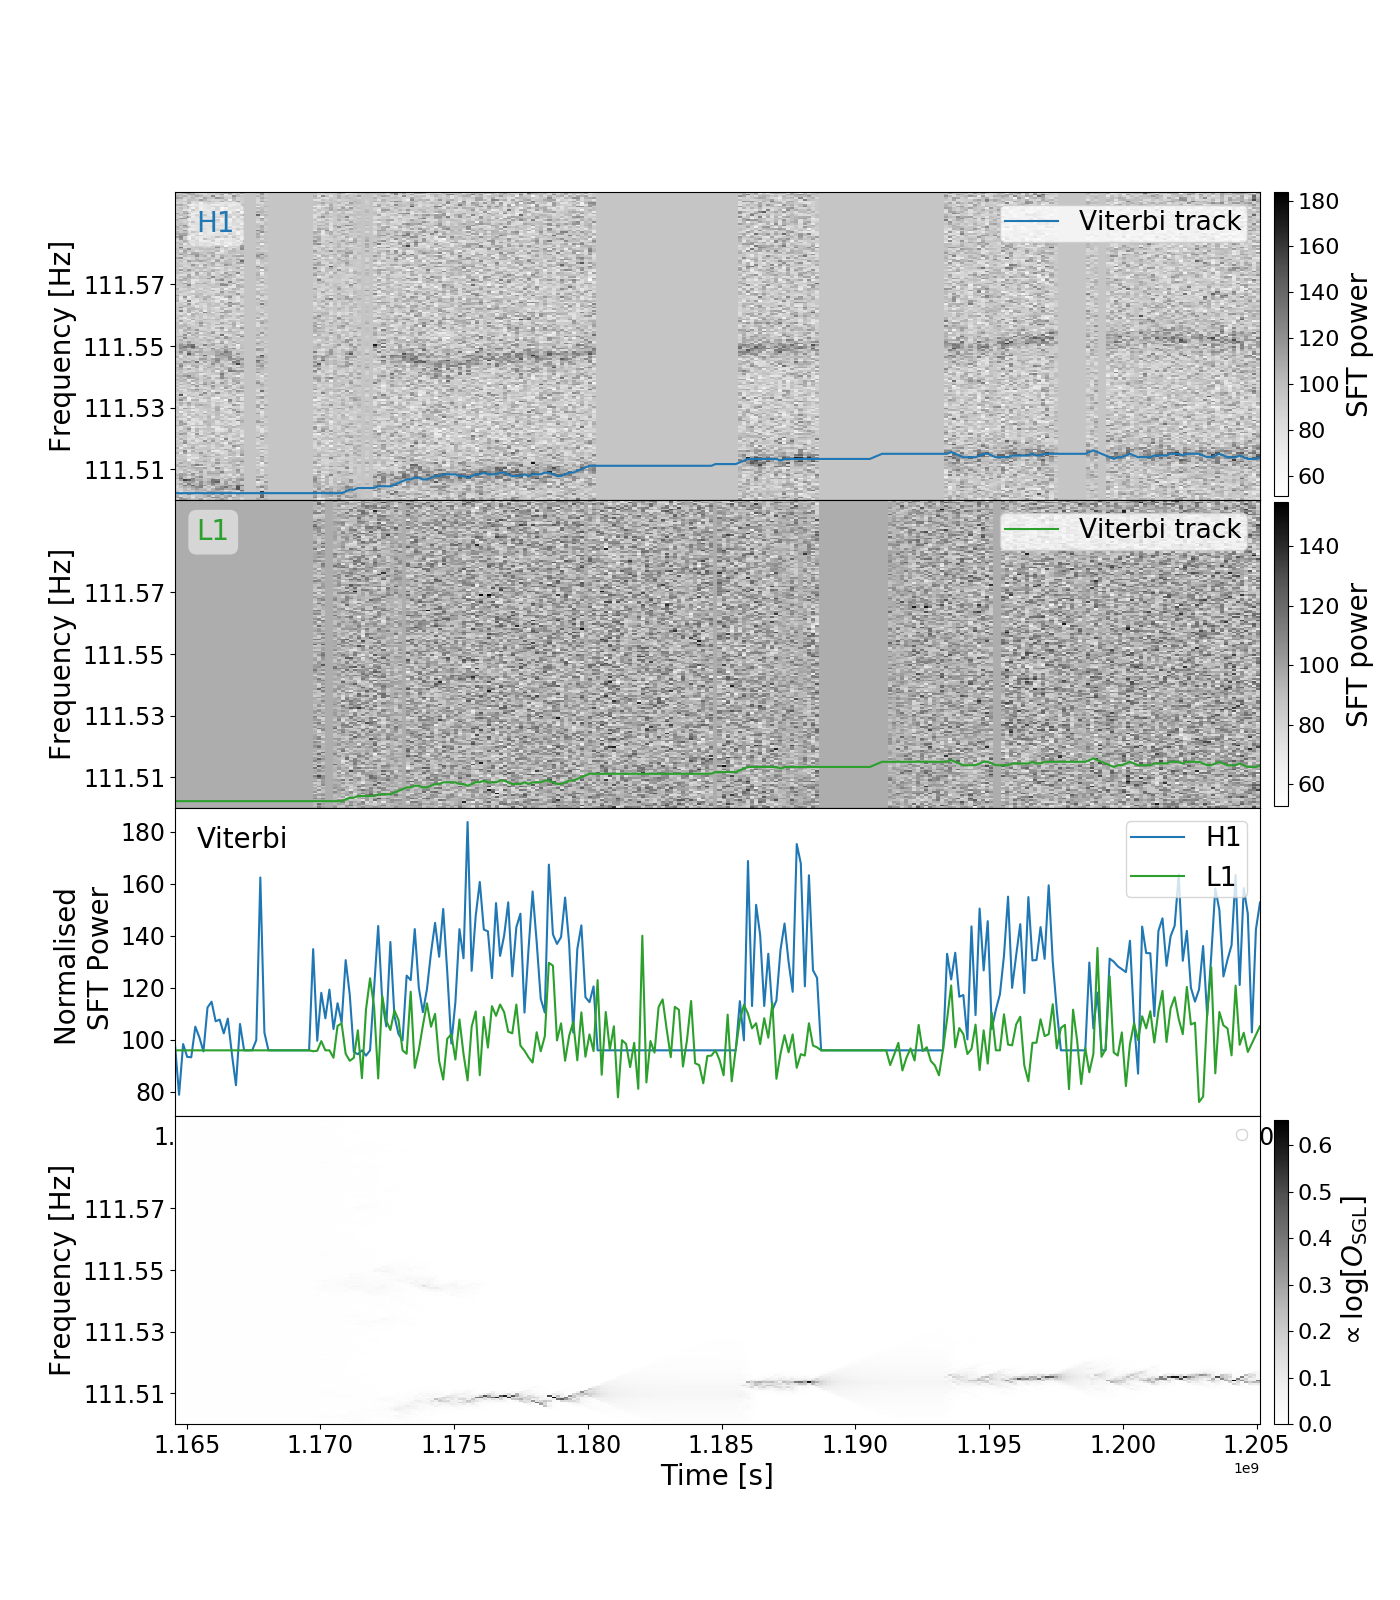
\includegraphics[width=\textwidth]{C6_detchar/plot_F111_5_wandering_line.png}
        \caption[Broad wandering line example.]{~\chris{Comment for all plots.
			Start with a descriptive sentence of hwt is being plotted.} Broader
			instrumental lines are generally weaker and can be mistaken for an
			astrophysical signal by the SOAP astrophysical search. Above an example of two
			broad lines in the H1 detector is shown, where SOAP has identified one of
			the~\chris{sort out this sentence. It's got grammar problems and isn't
			complete.}.
			The top two panels show the summed spectrograms from the H1 and L1 panels with
			the optimal Viterbi track overlaid. The third panel shows the normalised
			spectrogram power along the Viterbi track for each of the detectors. The final
			panel shows the Viterbi map for this frequency band.~\chris{I know that this is
			an astrophysical result plot but the colour scheme is quite differnet to the
			line search outputs from SOAP.}
			}
\label{detchar:soap:astrowander}

\end{figure}
%
Figure \ref{detchar:soap:astrowander} shows a broad and wandering line in a single
detector causing the SOAP search to mistake it for an astrophysical signal.
This is because the SOAP line aware statistic from Sec.~\ref{soap:las} finds
areas of higher power which are consistent between detectors according to the
parameters~\chris{according to the parameters is nebulous - be specific} of the
statistic. These types of line are difficult to mitigate in an astrophysical
search as there is consistent higher \gls{SFT} power in both the broad line and the noise in the other detector.
However, this has a side effect of being useful to identify the
instrumental lines themselves.
In this section, I will explain the setup of the search to identify
instrumental lines.

It is often useful to search through the auxiliary channels when trying to
identify the source or a line. 
This would involve using out multiple detector search in Sec.~\ref{soap:multidet} to identify lines which are coincident between channels. 
The aim of this section however, is to flag potential lines within the \gls{GW} channel.
Whilst we have developed a statistic in Eq.~\ref{soap:las:stat} to penalise line like signals, we revert to using the
`normalised' \gls{SFT} power as the statistic in the SOAP search. The single
detector search then has one parameter to vary, the transition matrix
parameter $\tau$.  This governs how probable the frequency track is to transition up,
straight or down a frequency bin.  In this search we are aiming to find any line-like artefact.
Therefore, we allow an equal probability for the track to jump in any
direction, but limit it to change by one frequency bin after each time
segment.  

Whilst the astrophysical search summed the \glspl{SFT} over one day
as shown in Fig.~\ref{detchar:soap:astrowander}, for the line search, we assume
that instrumental lines are stronger than astrophysical signals and therefore
should be identifiable in the raw 1800s long \glspl{SFT}.
A search could also be run on summed \glspl{SFT}, which may improve the sensitivity to weaker lines,.~\chris{possible
examiner question - what would happen if you did sum the data and do the line
search on summed power?}. The Fscan search
described above generates \glspl{SFT} which are 1800 s long (as well as some other lengths).  For this line search, we split the 1800 s
long Fscan \glspl{FFT} into 0.2 Hz wide sub-bands and run the single detector
search on each sub-band. A 0.2 Hz wide sub-band was chosen for this to reduce halve the number of output plots to save and further analyse, this however, could be reduced to 0.1 Hz if necessary.  The search then returns the same outputs as described in
Sec.~\ref{soap} and Sec.~\ref{machine}: the frequency track (Viterbi track), a
Viterbi map and a Viterbi statistic.  Here the Viterbi statistic is just the
sum of the \gls{SFT} power along the frequency track.  

The line search then outputs plots as shown in Fig.~\ref{detchar:soap:linewander},
\ref{detchar:soap:noiseplot}, \ref{detchar:soap:lineplot} and
\ref{detchar:soap:wanderplot}.  These plots and the equivalent plots for other
sub-bands can then allow each sub-band to be classified into containing an
instrumental artefact or not.  An example of the SOAP line search being run on
the H1 detector on the same instrumental line but with slightly wider frequency
band as Fig.~\ref{detchar:soap:astrowander} can be seen in
Fig.~\ref{detchar:soap:linewander}. This shows how the line search identifies
the same instrumental line albeit at a higher resolution and can flag it for
further investigation.~\chris{These last 2 sentences need some explaining. What
is the purpose of these plots and their comparison - you must expand upon these
kind of things! and why do they have different band widths? Also this is a beast of a paragraph - please break it
up.}
The final panel shows how the \gls{SFT} power of the signal along th Viterbi track varies with time, this shows how the \gls{SFT} power of the line was at a maximum at the end of June.
Also this shows the mean noise floor in this frequency band as a function of time, this should identify if the 

%
\begin{figure}[hpt]
	\centering
	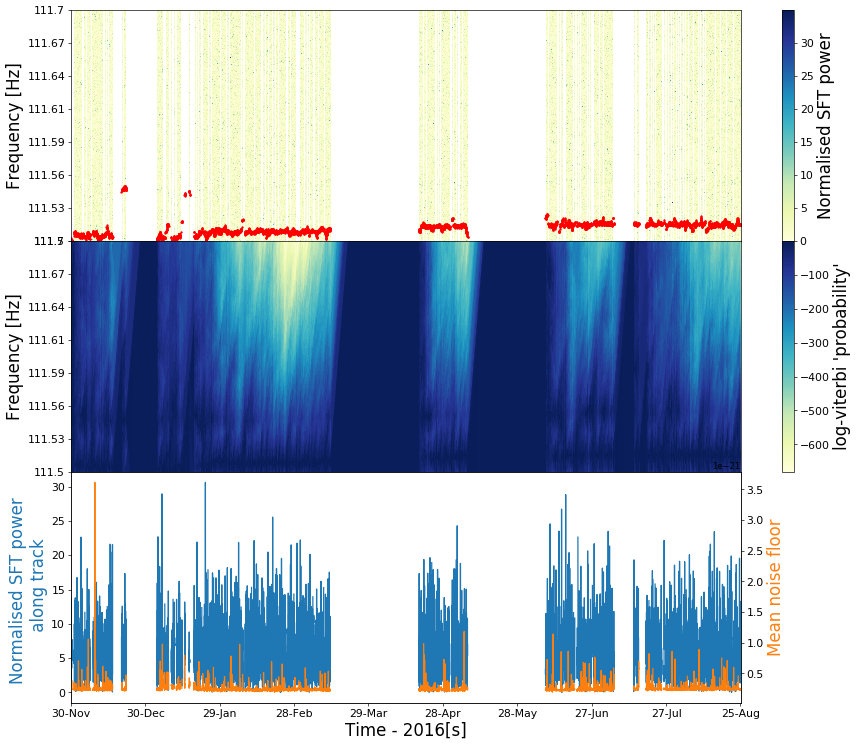
\includegraphics[width=\textwidth]{C6_detchar/track_F111_5_111_7_wander_2.png}
	\caption[Example SOAP output for wandering line]{\chris{start with a
general descriptive sentence. Also you need to describe all the features here
since it's not plotting the same things as Fig 5.2. Also, the colour scheme is
different to the astrophysical plots even though you plot some very similar
things.} The SOAP line search is run on a similar frequency band to Fig.~\ref{detchar:soap:astrowander}. This returns a similar track however at a resolution of 1800 s rather than one day.}
	\label{detchar:soap:linewander}
\end{figure}
%

\begin{figure}[hpt]
	\centering
	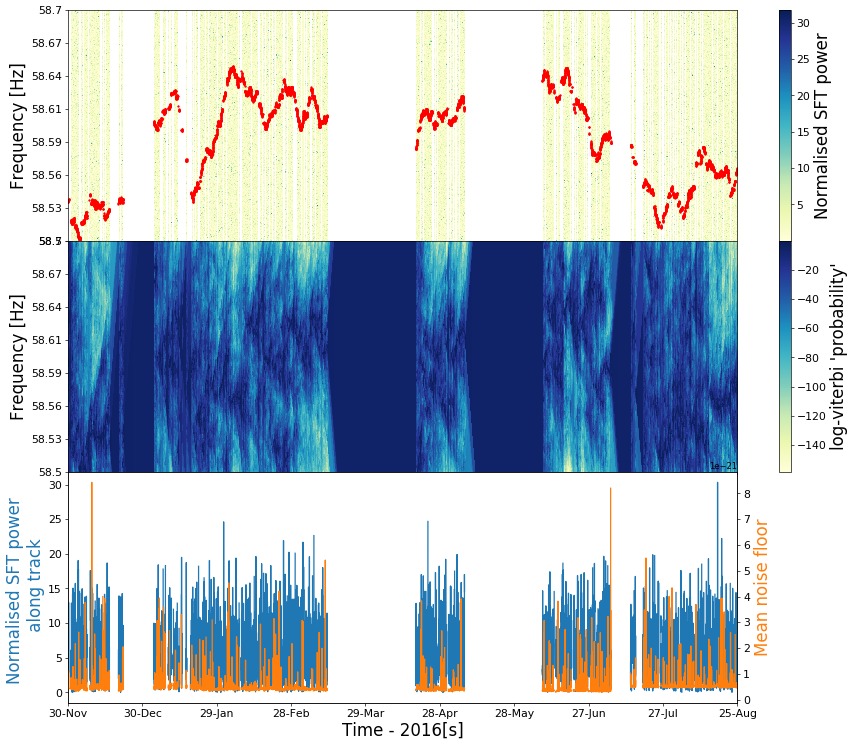
\includegraphics[width=\textwidth]{C6_detchar/track_F58_5_58_7_noise.png}
	\caption[Example SOAP output for Gaussian like noise.]{~\chris{the
descriptions you have here regarding the main aspects of what you are plotting
should be in the previous figure caption.}The SOAP search outputs three main
quantities, the Viterbi maps, the Viterbi track and the Viterbi statistic. The
Viterbi track is shown above overlaid onto the 1800s \gls{SFT} power spectrum
including the detector gaps for \glspl{LIGO} Hanford detector (H1) in its
second observing run (O2) \citep{}. This track is an indicator as to what type
of signal the track is following. The above track indicated that this is just
noise. The returned Viterbi statistic is also consistent with that of noise.
The Viterbi map is another visualisation of the sub-band, how to interpret this
has been explained in previous sections. However, here there does no appear to
be a clear signal. The final panel is a way to visualise how the \gls{SFT}
power changes along the Viterbi track. Also on this plot is an estimate of the
mean noise floor for this band to visualise how the sensitivity of the detector
changed over the course of the run.~\chris{be careful to stay descriptive in
the captions and to leave any interpretation of the figures to the main text
when you refer to the plot.}}

	\label{detchar:soap:noiseplot}
\end{figure}
%
Figure \ref{detchar:soap:noiseplot} shows an example of the spectrogram of a
sub-band which does not contain any signal or spectral artefacts but is
Gaussian distributed noise.  The track in the top panel of this plot shows the
power spectrum including detector gaps from 1800 s \glspl{SFT} in \gls{LIGO}
Hanford's data from its second observing run (O2).  The Viterbi track is
appears to be randomly wandering and is spread over the entire band, indicating that there is no astrophysical signal
present. 
 The Viterbi map plot does not show much
structure and contains areas of low log-probability.  Using this information
along with the Viterbi statistic result, this particular sub-band can be
considered to not contain an instrumental artefact. 
%
\begin{figure}[hpt]
	\centering
	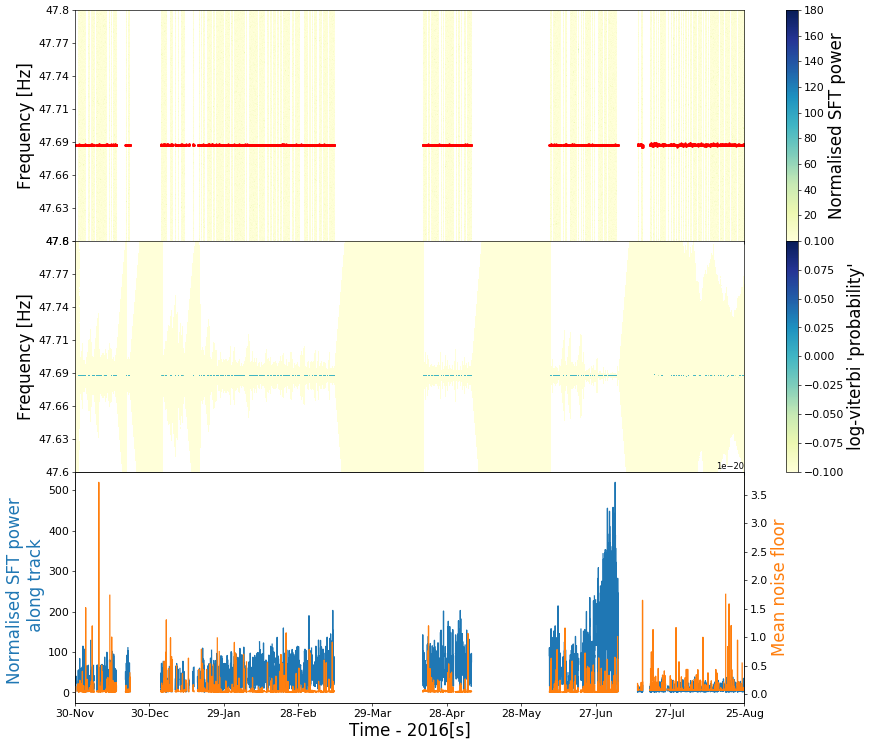
\includegraphics[width=\textwidth]{C6_detchar/track_F47_6_47_8_linenarrow.png}
	\caption[Example SOAP output for string narrow instrumental line.]{The equivalent plot as in Fig.~\ref{detchar:soap:noiseplot} can be made when there is a narrow spectral artefact in the band. The above is again results from \glspl{LIGO} Hanford detector (H1) in its second observing run (O2) using 1800s \gls{SFT} power spectrum. In this there is a narrow spectral line at $\sim 47.69$ Hz. The Viterbi track then follows this line of high power. The Viterbi map has much higher values for the log-probability in this line case compared to the noise case, this is an indicator some real signal. The probability in the Viterbi maps drops to zero in some areas due to the strength of the instrumental line. }
	\label{detchar:soap:lineplot}
\end{figure}
%

Figure \ref{detchar:soap:lineplot}
show a separate sub-band to Figure \ref{detchar:soap:noiseplot} which contains a strong and narrow
instrumental line.  The Viterbi track
does not have much spread over the band and stays at an approximately fixed
frequency, implying that this is a narrow spectral artefact.  
The Viterbi map plot then shows areas of high log-probability along the Viterbi track. The areas of white in the Viterbi
maps area areas where the probability of a signal falls to zero.  These pieces
of information along with the large value of the Viterbi statistic indicate
that there is a narrow spectral artefact within the sub-band.
The final panel shows how the \gls{SFT} power of the line was at a maximum at the end of June, and the sensitivity of the detector stayed relatively constant in this band.

%
\begin{figure}[hpt]
	\centering
	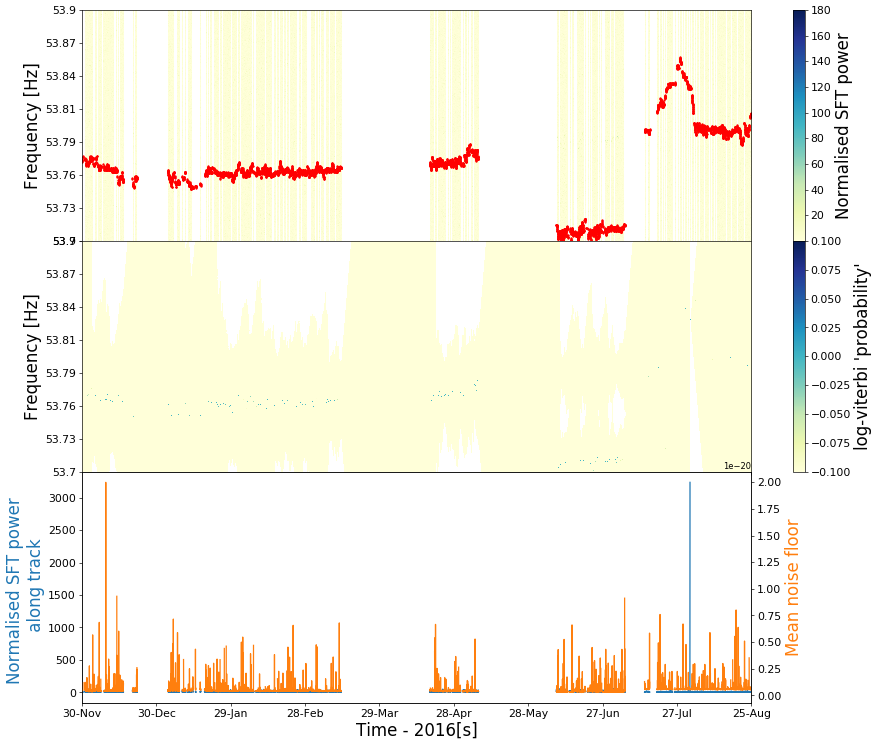
\includegraphics[width=\textwidth]{C6_detchar/track_F53_7_53_9_wander.png}
	\caption[Example SOAP output for wandering line.]{The equivalent plot as in Fig.~\ref{detchar:soap:noiseplot} can be made when there is a wandering spectral line. The above is again results from \glspl{LIGO} Hanford detector (H1) in its second observing run (O2) using 1800s \gls{SFT} power spectrum. This shows how some spectral lines do not have a fixed frequency bin can wander through the band. These are especially hard to track and monitor. The Viterbi track here shows is clearly different from the noise case in Fig.~\ref{detchar:soap:noiseplot} as the track is more tightly concentrated around some areas of power. }
	\label{detchar:soap:wanderplot}
\end{figure}
%

Figure \ref{detchar:soap:wanderplot} shows the equivalent plots to
Fig.~\ref{detchar:soap:noiseplot} and \ref{detchar:soap:lineplot} but now
contains a wandering spectral artefact.  This is
a line which wanders in
frequency as is moves though time.  This can be seen in the frequency
track, which here does not have much spread, however, the frequency of the
track changes with time.  There are also areas where the track switched to a separate spectral artefact within the same
band. This is where there are, for example, two instrumental lines within the same frequency band. The Viterbi algorithm will identify both of these and try to find a single track through the time-frequency spectrogram which given the highest sum of \gls{SFT} power. This could involve the algorithm using power from both of the lines at different times to build more \gls{SFT} power, the optimal track would then lie on both lines at different times. Fig.~\ref{detchar:soap:wanderplot} shows this discrete jump around
January.~\chris{you have to allow the reader to understand these concepts
slowly. You are very abruptly introducing the concept of tracks switching but
you must explain in more detail what you mean by this.} 

The combination of the Viterbi statistic, Viterbi map and spectrograms are then
used to flag any given sub-band as
containing a possible instrumental
artefact.  Figures \ref{detchar:soap:linewander},
\ref{detchar:soap:noiseplot}, \ref{detchar:soap:lineplot} and
\ref{detchar:soap:wanderplot} show some specific
examples of lines, however, there is a lot of variation in the types of lines and
features which appear in all of the SOAP outputs.  This line search then works
by initially ranking all of the Viterbi statistics.
Larger values of the Viterbi statistic are good indicators that there is an instrumental line present within the sub-band. 
Larger Viterbi statistic's indicate that there is a tracks of high \gls{SFT} power within the sub-band, which is a similar signature to an instrumental line.

Figure~\ref{detchar:soap:rankedstats} shows an example of a
histogram of the ranked Viterbi statistics from O2. 
%
\begin{figure}[ht]
	\centering
	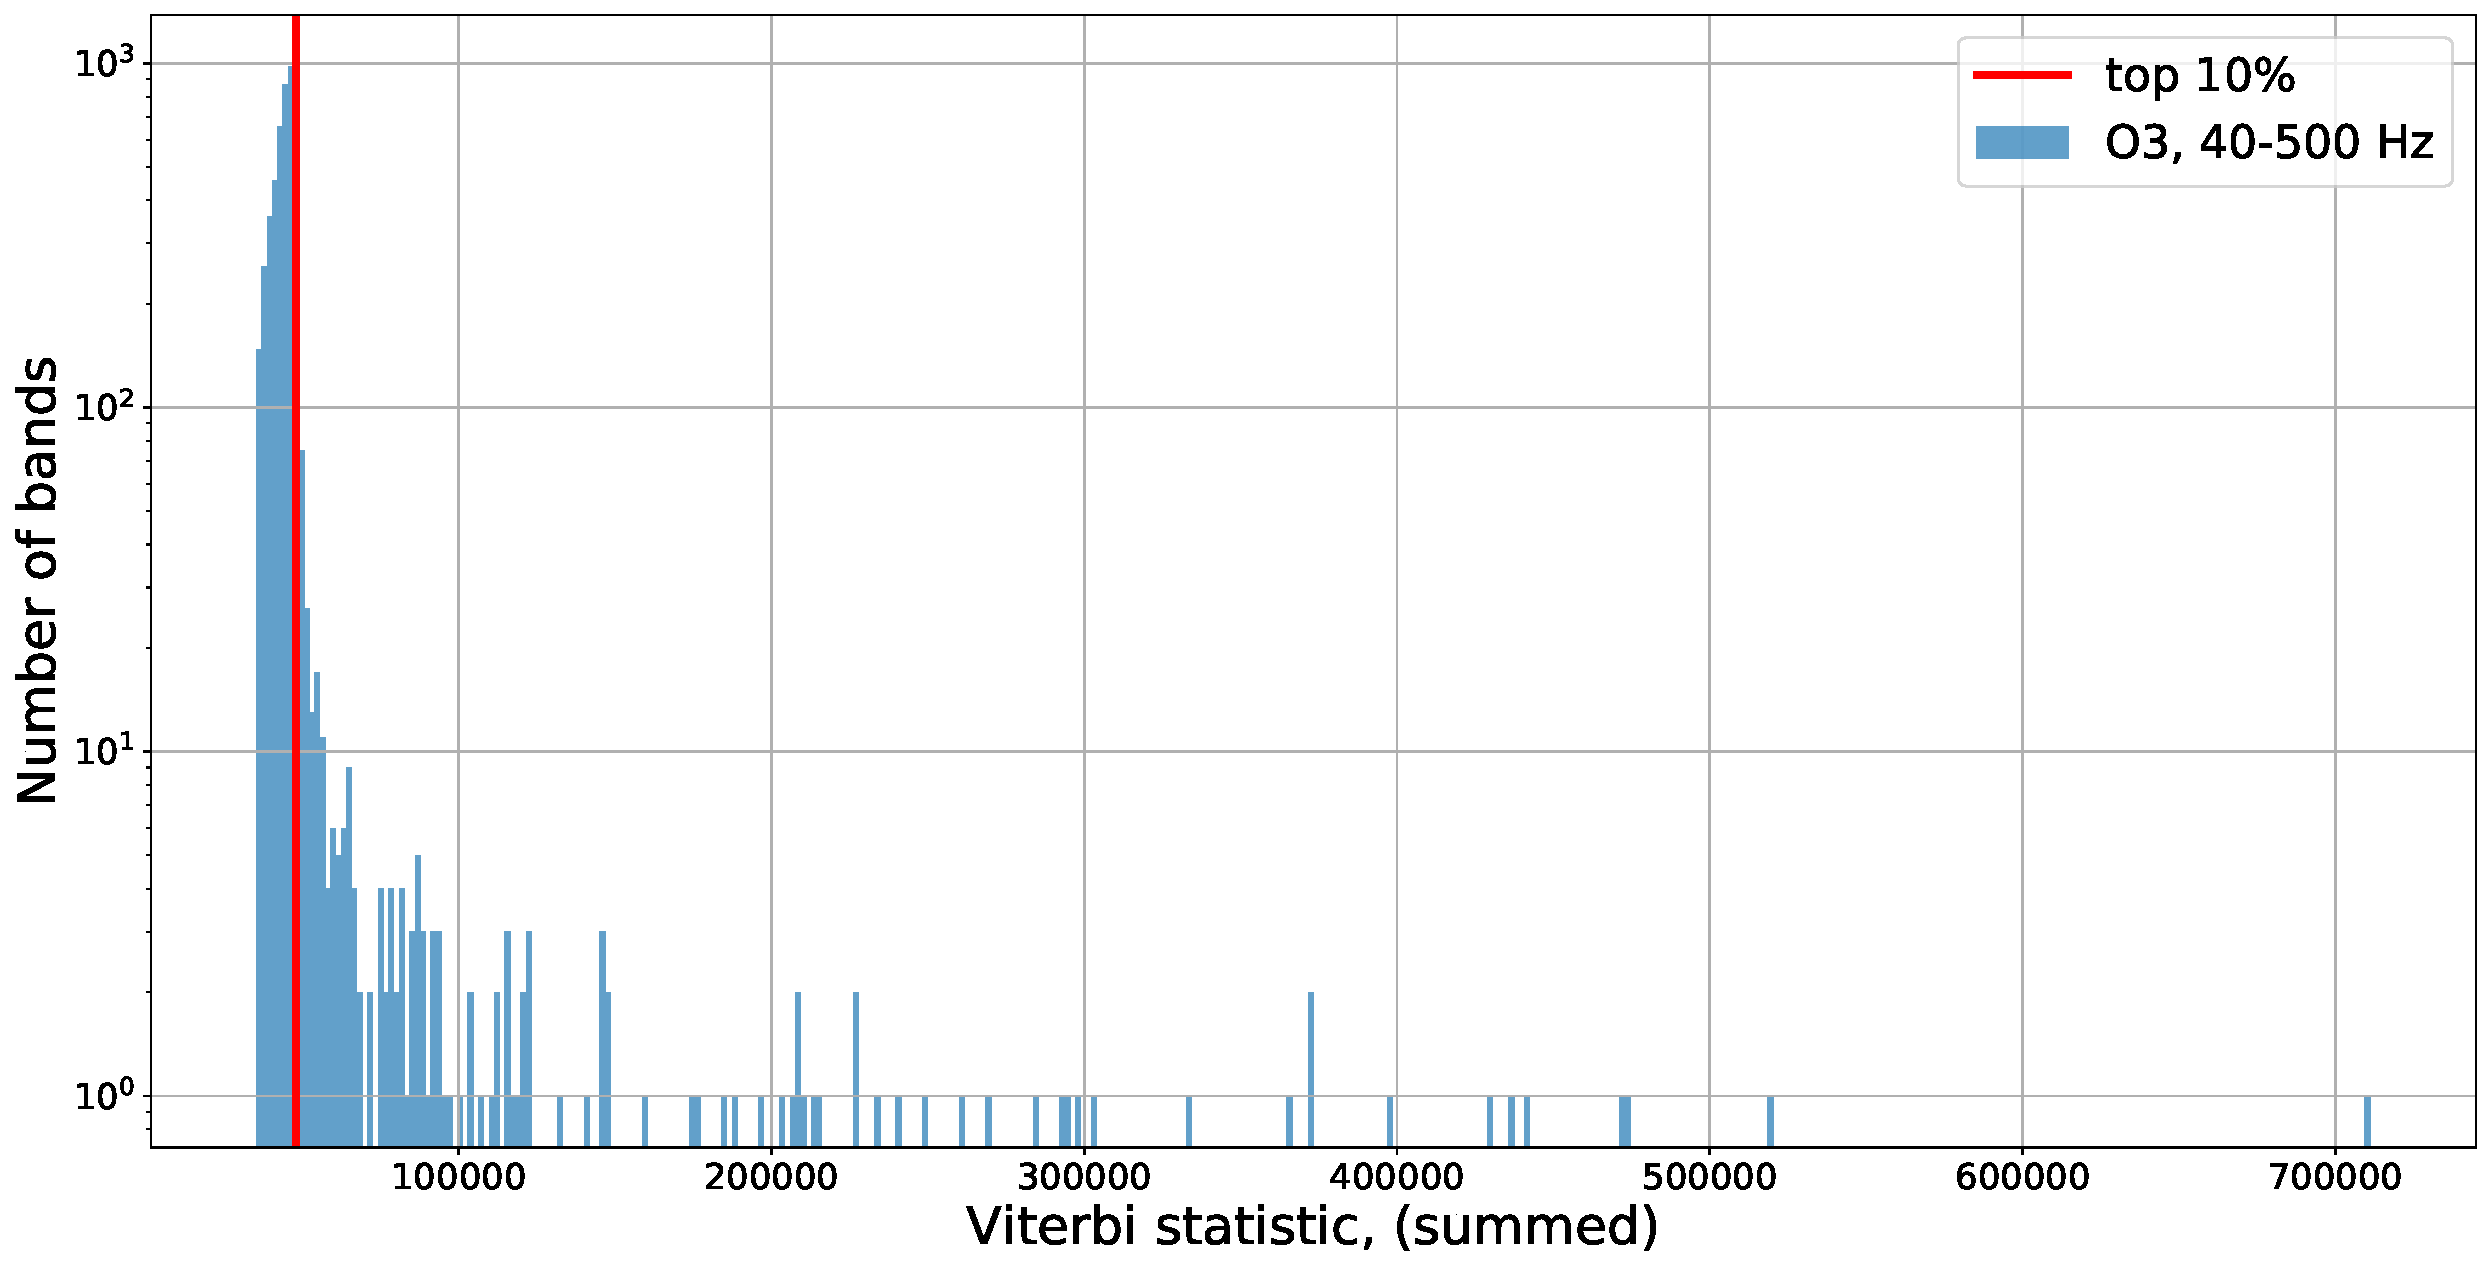
\includegraphics[width=\textwidth]{C6_detchar/statistic_hists_O3_H1.pdf}
	\caption[Viterbi statistics for H1 in O3]{\joe{change to O2} }
	\label{detchar:soap:rankedstats}
\end{figure}
%
The sub-bands which give statistic
values which lie outside the main distribution can then be viewed for further
investigation. The high values outside the distribution are currently defined
rather arbitrarily, this could either be something like the top 10\% of
sub-bands or could involve looking through the ranked list until signals begin
to look like noise~\chris{this thesis is not an informal discussion - you need
to sound authoratative on your topic. Make a decision on how to rank things,
motivate it and stand by it}. The top results which are deemed to come from an
instrumental line~\chris{ambiguous - are top results from lines or are a subset
of results
from the toplist deemed to be lines?} can be compared to the known line lists from the other line
tools mentioned in Sec.~\ref{detchar:monitor}.  Any new lines can be
investigated further by methods described in
\citep{covas2018IdentificationMitigation} using the tools in
Sec.~\ref{detchar:monitor}.  A list of lines which have been categorised by
these searches can be found here in {\tt
\url{https://ldas-jobs.ligo-wa.caltech.edu/~evan.goetz/CW/O3aLines/H1/index.html}}
and lines which have not been categorised in {\tt
\url{https://ldas-jobs.ligo-wa.caltech.edu/~evan.goetz/CW/O3aLines/H1/Unidentified/index.html}}~\chris{what
does not being categorised mean in relation to those that have been
categorised? Please expand on this. Why is it important?}.
The two line lists above can then be compared to the output of the SOAP line
search.~\chris{and?}


When running this search SOAP identified lines which did not appear in other
line lists, therefore, offers a method to search for weaker lines.
\joe{actually check this}~\chris{Yes, if you are able to compare line lists and
identify lines that you have but that are not on the offical line list then you
should make some plots of them and discuss.}

\joe{need to mention why this is good as extra tool, i.e. searching for wandering lines, identifies track of very weak lines etc, things that other searches cannot do}

\clearpage 
%%%%%%%%%%%
%%%%%%%%%%%%
\section{\label{detchar:summary}Summary pages}
%%%%%%%%%%%
%%%%%%%%%%%%%

Summary pages are an important tool when searching for instrumental lines.
There is such a large amount of data both in frequency and time space, and
channels to search though when looking for instrumental lines~\chris{clunky
grammar}. Summary pages
distill this data such that only the important information is shown. This
enables lines to be identified easily when looking through sub-bands. The
criteria when designing summary pages is that they are easy to navigate and the
important information is shown in a clear and concise way.  How we display this
information will be explained later in this section.  These summary pages exist
for the above searches~\chris{so you have summary pages for the astro searches
too? This section seems to imply that summary pages are only useful for
instrumnental line searches - please resolve.} in \citep{bayleyHome} where this is only accessible by
\gls{LIGO}~\chris{and Virgo and KAGRA} members.

For the SOAP search summary pages were generated~\chris{grammar} for each observing run and for
the two \gls{LIGO} detectors~\chris{why not Virgo?}. This was done for various timescales: for the
entire observing run and separately for each month.  This allows the variation
of a line to be observed for the entire length and also artefacts on shorter
timescales~\chris{clunky grammar} to be observed. Once the detector, observing
run, and timescale is
set, the band~\chris{what band?} is split into 0.2 Hz wide sub-bands.  The Viterbi search with a
flat transition matrix and using the summed \gls{SFT} power as the
statistic~\chris{this sentence has no conclusion. It also mentions the summed
SFTs but I thought you don't use that for the lines?}.
A flow diagram of how the SOAP search works for instrumental line searches can
be found in Fig.~\ref{detchar:summary:flow}.
%
%
\begin{figure}[hp]
	\centering
	

\tikzstyle{block} = [rectangle, draw, fill=blue!20, 
    text width=17em, text centered, rounded corners, minimum height=4em]
    
\tikzstyle{line} = [draw,line width=0.35mm, -latex']


\begin{tikzpicture}[node distance = 6em, auto]

    % Place node
    
  	\node [block] (sft) {1.\\ SFTs from Time series};
  
  	\node [block, below of=sft] (norm) {2. \\ Divide \gls{SFT} by running median and get power spectrum.};
  	\node [block, below of=norm] (narrow) {3. \\ Narrowband \gls{SFT} (0.2 Hz)};
	
	\node [block, below of=narrow] (soap) {4. \\ Run SOAP search and generate plots};
  
   \node [block, below of=soap] (summary) {5. \\ Generate summary page};

  
  % Draw edges
  \path [line] (sft) -- (norm);
  \path [line] (norm) -- (narrow);
  \path [line] (narrow) -- (soap);
  \path [line] (soap) -- (summary);
  

  
    
\end{tikzpicture}
	
	\caption[Flow diagram for SOAP line search.]{\label{detchar:summary:flow} The SOAP search for instrumental lines is simpler than other searches. A simple version of the search is run separately for each detector, where the raw \glspl{SFT} are divided by their running median, narrow-banded and then the search is run. }
	
\end{figure} 
These stages are as follows:
\begin{description}
	\item[1. \glspl{SFT} from time series] The \glspl{SFT} are generated for the \gls{GW} output channel. This is done by the Fscan search, therefore we do not repeat this process. Currently the search only runs on the \gls{GW} channel, however, in the future could be made to run on others.
	
	\item[2. Divide \gls{SFT} by running median] In this stage each
\gls{SFT} is divided by its running median~\chris{as discussed before, we don't
only divide by the running median because that would leave our data with median
= 1. We apply a correctiuon factor to make the mean=1 even though we divided by
the mnedian. Alos, we don't devide the SFTs by the median, we divide the SFT
power by the median - an important distinction.} which is 100 bins
wide~\chris{why is choice made?}. The running median takes each \gls{SFT} and
applies a window of 100 bins, where the median of these 100 frequency bins is
taken~\chris{repeated use of 100 bins}. This window then slides over the
\gls{SFT} producing an `filtered' \gls{SFT} which should exclude
outliers.~\chris{No. The filtering by the running median is a essentially a
high pass filter than cuts out broad (low frequency) bumps in the noise
variation in the frequency dimension. Outliers are not removed.}
	
        \item[3. Narrow-band \gls{SFT}] The \gls{SFT} is then split into 0.2 Hz
wide sub-bands for the SOAP search to run on. These smaller bands are chosen as
the SOAP search pull~\chris{pull?} information on the most likely track, therefore, smaller
bands are not contaminated by areas of high power in neighboring frequency
bands. 
	
        \item[4. Run SOAP and generate plots] This stage runs the SOAP search
with a flat transition matrix probability and generates plots as shown in
Fig.~\ref{detchar:soap:noiseplot}.
	
        \item[5. Generate summary page] Finally the summary pages~\chris{you
are assuming that the reader knows that summary pages are actual pages and are
stored and viewed online. It might seem obvious to you but think about the
reader.} are built
which take all of the bands and puts them in a table. This table can be ordered
by the value of the Viterbi statistic, or can be searched for particular
frequency bands.  
\end{description}

An example of a summary page is shown in Fig.~\ref{detchar:summary:plots}. This
has been annotated showing how to navigate the page.  There are generally two
separate parts to the page: selecting the observing run and frequencies, and
viewing the outputs.  The observing run is selected at the top of the page,
where currently this has only~\chris{no need to downplay, just say that it has
been run on O2 and O3} been run on O2 and O3.  From this menu the
detector can be selected, currently only \glspl{LIGO} H1 and L1 detectors are
present. The selection of frequencies and viewing of outputs then happens on
this page~\chris{strange sentence}. The key information of each page is the plots shown in
Figs.~\ref{detchar:soap:linewander} - \ref{detchar:soap:wanderplot}.  These
clearly show the data with a number of representations of the data~\chris{data
and data}. They show
the time frequency spectrograms of the data, the output Viterbi tracks which
identify the most probable frequency track, the Viterbi maps which allow the
probability of a signal as a function of the time and frequency bin to be
viewed.  Finally they show the spectrogram power along the Viterbi track with
the mean noise floor of the detector during the observing run.  This should
provide enough information to determine whether an instrumental line in
present.~\chris{Really? It shoud certinaly provide a useful set of information
to assess the prsence of a line.} To navigate each page, the left panel contains a calendar where the
start and end times of a result can be selected.  Currently there are
pre-defined times which can be selected from. This allows a line to be
investigated for a shorter or longer time period.  This can be useful when a
new instrumental line appears and it needs to be investigated only from when
the line appears.  Below this in the left panel of the page there is a table
where each cell is one of the sub-bands which was searched through. This allows
individual frequency bands of interest to be searched for as well as the table
to be limited between different frequencies.  The table contains four columns:
the frequency of the sub-bands, the Viterbi statistic, the $\sigma$ from the
mean of all the sub-band Viterbi statistics and extra information.  The first
two columns are self explanatory, the frequency range of the sub-band and the
resulting Viterbi statistic from that sub-band. The table can be ordered by the
Viterbi statistic such that only the highest values are investigated.  The
$\sigma$ from the mean is found by approximating the distribution of the
Viterbi statistics as a Gaussian.  A Gaussian is then fit to the distribution
using a simple least squares, each statistic then has a multiple of $\sigma$
away from the mean of this distribution.  This is an approximate calculation to
give a scale of how significant the statistic in that sub-band is.  The final
column contains any extra information which exists for that particular
frequency range.  For example, this is filled with other line list information
which has been collected from other search methods.  The loud features such as
Violin modes can then be marked. This means that these particular bands are
likely to have been investigated already allowing this search to focus on any
extra instrumental lines.~\chris{Nice descriptions. It's another monster
paragrpah so please break it up.}



\begin{sidewaysfigure}[p]
	\centering
	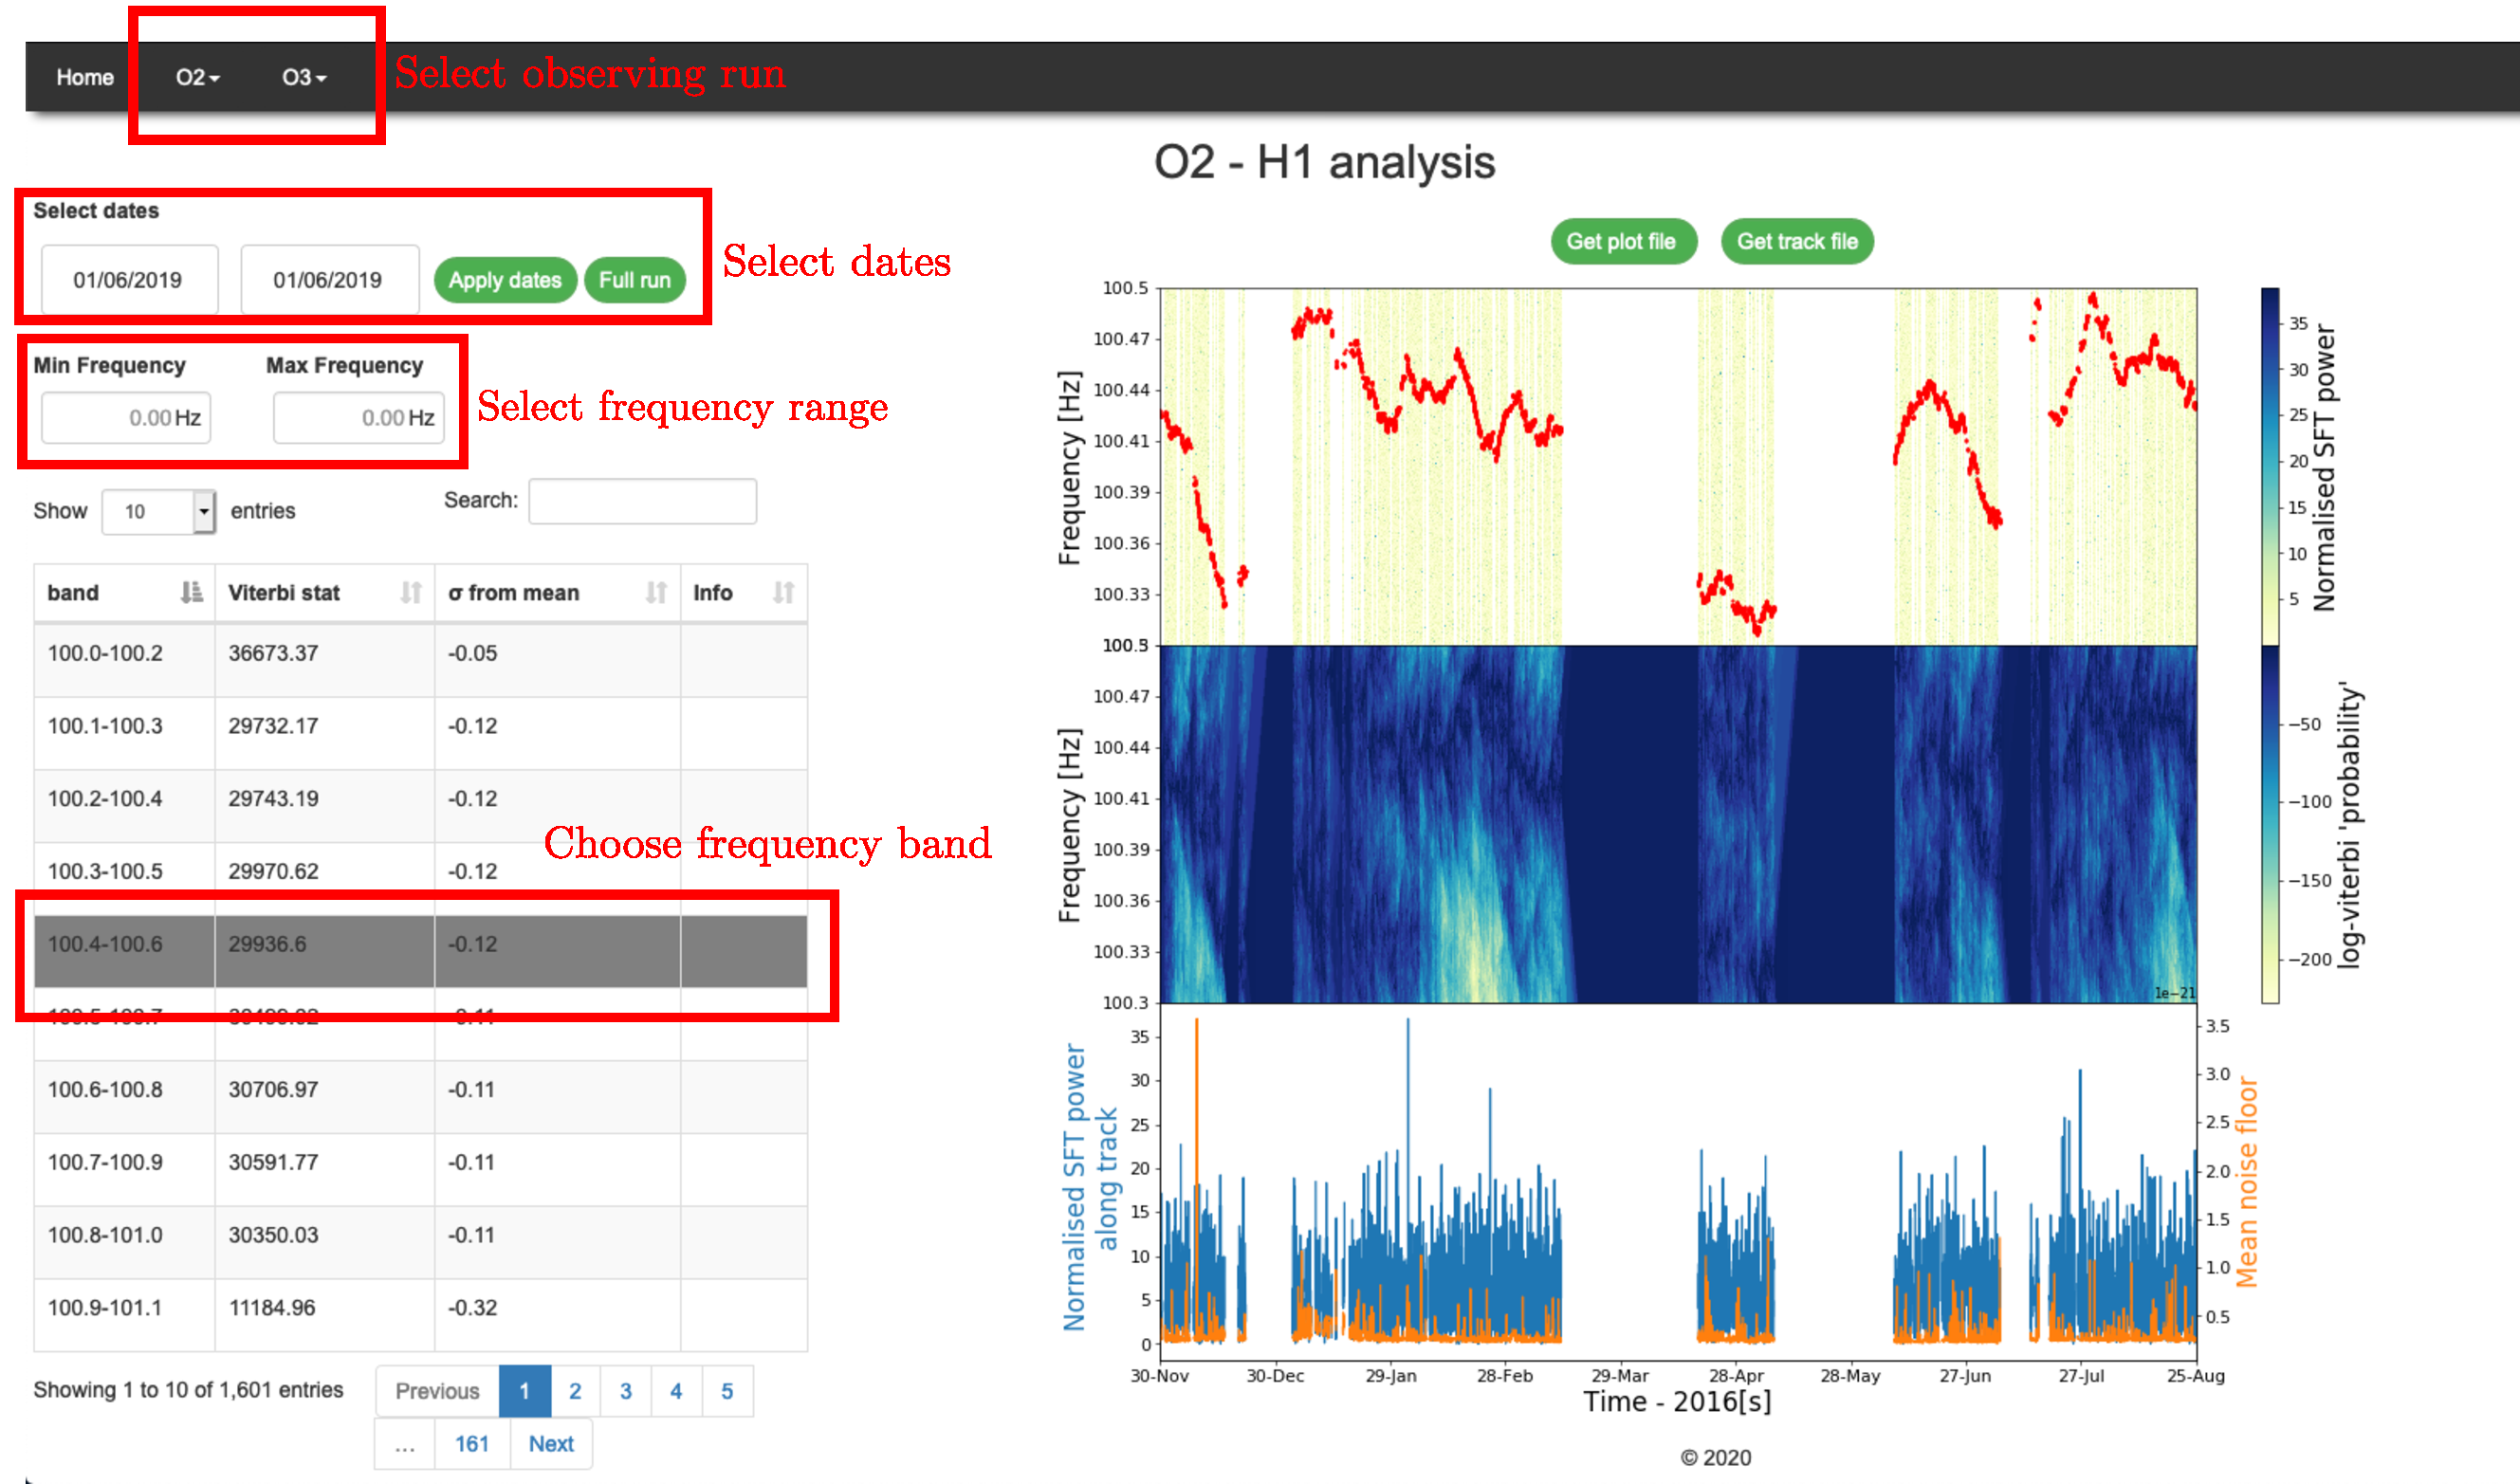
\includegraphics[width=\textwidth]{C6_detchar/summary_annot.pdf}
	\caption[Example summary page for SOAP search]{The summary pages are made for each observing run (in this case just O2 and O3). The range of times can then be selected from a set of start and end times. This is in general the entire observing run and monthly runs of this search. These pages can be found at \citep{bayleyHome}}
	\label{detchar:summary:plots}
\end{sidewaysfigure}

The summary pages are then hoped to be useful alongside the other tools for
searching for instrumental lines. \joe{more}~\chris{yes, I agree, a bit more
would be good. Also you need to beef up the references. You only have $\sim 6$
on detchar at present.}


\clearpage

%%%%%%%%%%%
%%%%%%%%%%%
\section{Armadillo}
%%%%%%%%%%%
%%%%%%%%%%%

Armadillo was a project which aimed to develop a diagnostics tool to be used at the \gls{LIGO} detectors.

\begin{itemize}
	\item LIGO has large control systems
	\item these can be generally split into two parts: Analogue and digital control systems
	\item Armadillo was a tool that focusses on the digital control system
	\item Having an understanging of what happens to a signal as it passes through the control system is important it can help identify source of glitches
	\item one way to do this is to look at the transfer funtion of a possible signal path 
	\item Armadillo aimed to find a simple way to return the transfer function between any two points in the control system.
\end{itemize}


To find the transfer function between any two points in the digital control system, one needs to know all the possible paths a signal could take between those two points and each of the component filters which lie along the paths.
The models of the digital control system for \gls{LIGO} are stored in Simulink diagrams \citep{}.
These generally 

\begin{itemize}
	\item May components are need to explain a transfer function
	\item first step is to load all the models from simulink diagrams
	\item these contain of many blocks and connections see Fig ....
	\item each block can be a single filter or a submodel which contains many more filters
	\item there is then a large number of filters and possible paths
	\item for each filter, one needs to load the `FOTON' filter files which contain the coefficients 
	\item there are also blocks which are matricies which only allow a signal to pass along a certain path at a given time
	\item These are defined int EPICS by the user, and their values at any time are stored
	\item 
\end{itemize}
